%!TEX root = ../../thesis.tex


\section{Deriving the Radial Velocity}

RV derivation...
Eliptical orbit



Radial Velocity:
Picture of orbital motion.
Concepts of {RV} motion-
Masses,
Orbits, (period, mass, distance impact.)
Equation
What the Equations mean.
\begin{figure}
    \centering
    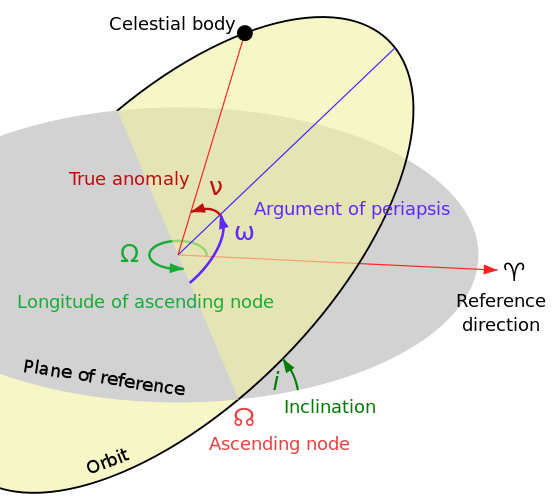
\includegraphics[width=0.5\linewidth]{figures/advanced_material/orbit}
    \caption{By Lasunncty at the English Wikipedia, CC BY-SA 3.0, \href{https://commons.wikimedia.org/w/index.php?curid=8971052}{https://commons.wikimedia.org/w/index.php?curid=8971052}}
    \label{fig:orbit}
\end{figure}


\subsection{{RV} calculation}
\unfinished{Move location / adjust from paper}
We use the Keplerian orbit {RV} equation to estimate the {RV} of the host and companions at the time of each observation, \(t\):
\begin{equation}
\label{eqn:rv_equation}
{RV} = K [\cos{(\nu(t) + \omega)} + e\cos{(\omega)}]
\end{equation}
Here, \emph{K} is the \emph{semi-major amplitude}, \(\nu\) is the \emph{true anomaly}, \(e\) is the orbital \emph{eccentricity}, and \(omega\) is the \emph{argument of periastron}.
The true anomaly is not only a function time, \(t\), but also the orbital period \(P\), the \emph{time of periastron passage}, \(T_0\), and eccentricity.
The literature parameters for each target are provided in \cref{tab:orbitparams}.
To determine the {RV} of the companion we transformed the {RV} semi-amplitude of the host \(\kone\) into the semi-amplitude for the companion \(\ktwo\) using the mass ratio,
\begin{equation}
\label{eqn:mass_ratio}
q = \mtwo / \mone = \kone / \ktwo
\end{equation}

We note that for the targets in which only the minimum mass (\mtwosini) is known, this equation will indicate the maximum \(\ktwo\) value for the companion. The estimated \(\ktwo\) for each companion is provided in \cref{tab:estimatedparameters} while the {RV} for both components at the time of each observation is provided in \cref{tab:observations}.


\todo{Possibly just move this too the plae where it is used.}
The error on estimated {RV} values, shown in \cref{fig:HD211847_result_contours}, is calculated by applying the general error propagation formula~\citep{ku_notes_1966} and using the errors on the orbital parameters. For a function, \(f\), with errors on the inputs \(\delta x\), \(\delta y\) etc., it follows:
\begin{align}
f &= f(x, y, z, \ldots)\\
\delta f &= \sqrt{{\left( \frac{\partial f}{\partial x} \delta x\right)}^2 + {\left(\frac{\partial f}{\partial y} \delta y\right)}^2 + {\left(\frac{\partial f}{\partial z} \delta z\right)}^2 + \ldots}.
\end{align}




% from draft of paper 18/7/2017
\subsection{Companion K}  Maybe something can go above from this...
\label{sec:companion_RV}
\emph{These sections might be unnecessary}\\

To calculate the {RV} of the companion at the time of each observation. For a two-body system the {RV} semi-amplitude of the companion \(\ktwo\) can be determined from the orbital host-companion mass ratio
\begin{equation}
q = \mone/\mtwo = \ktwo/\kone\label{eqn:q_ratio_K2}.
\end{equation}
Note, that for the targets in which only the minimum mass (\mtwosini) is known, this will give the maximum {RV} semi-amplitude of the companion.
This relation was used to estimate \(\ktwo\) for the companion from the minimum mass or mass we have for each companion. These values along with the other orbital parameters of the system were used to calculate the {RV} of the companions for each observation. These values are provided with the observations in \cref{tab:observations}.




If more than one planet is present then they gravitational influence each other and their orbits become non-Keplerian, i.e.\ a N-body problem? {\textbf{ref}}. In this work were a star has two companions we will only assume Keplerian orbits from individual planets, independently.
